\documentclass{ctexart}

% 中文支持由 ctexart 文档类自动提供

% 页面设置
\usepackage[top=2.54cm, bottom=2.54cm, left=3.18cm, right=3.18cm]{geometry}

% 数学公式
\usepackage{amsmath, amssymb, amsthm}

% 图形与表格
\usepackage{graphicx}
\usepackage{float}
\usepackage{booktabs}

% 列表与线路图（用于 4(d) 详解）
\usepackage{enumitem}
\usepackage{tikz}
\usepackage{xcolor}

% 超链接
\usepackage{hyperref}

% 量子态和算符
\usepackage{bm}
\newcommand{\ket}[1]{|#1\rangle}
\newcommand{\bra}[1]{\langle #1|}
\newcommand{\braket}[2]{\langle #1|#2\rangle}

% 标题设置
\title{Problem 1: Preliminaries and Warm-up\\[4pt]\large 完整合并解答}
\author{}
\date{\today}

\begin{document}

\maketitle

\noindent
\textbf{说明：} 本文档以 \texttt{Problem1-Solution.tex} 的题面与排版格式为骨架，汇总了第 1 题各小问的全部解答，来源如下：第 1--3、6 题取自 \texttt{Problem1-Solution.tex}；第 4 题取自 \texttt{problem1(1-4done).tex}，并附 4(d) 的最优线路与下界详解（取自 \texttt{problem1\_4d\_answer.tex}）；第 5 题取自 \texttt{Problem1(1-5done).tex}；第 7、8 题依据 \texttt{code/} 下对应代码（\texttt{problem7\_reversible.py}、\texttt{8\_grover.py}、\texttt{quantum\_circuits.py}）整理。数值/线路验证脚本见 \texttt{code/} 目录，测量线路图见 \texttt{figs/} 目录。

\medskip

\section*{Problem 1: Preliminaries and Warm-up}

\subsection*{1.}
Show that $R_{\mathbf{n}}(\theta) = e^{-i\frac{\theta}{2}\mathbf{n}\cdot\boldsymbol{\sigma}}$ takes the form
\begin{equation}
    \cos(\theta/2)I - i\sin(\theta/2)(n_X X + n_Y Y + n_Z Z),
\end{equation}
where $\mathbf{n}$ is a unit 3D vector and $\boldsymbol{\sigma} = (X, Y, Z)$.

\medskip
\noindent\textbf{Solution:}
首先计算 $(\mathbf{n}\cdot\boldsymbol{\sigma})^2$。Pauli 矩阵满足对易关系
$\{X,Y\} = \{Y,Z\} = \{Z,X\} = 0$ 和 $X^2 = Y^2 = Z^2 = I$，因此
\begin{align*}
    (\mathbf{n}\cdot\boldsymbol{\sigma})^2
    &= (n_X X + n_Y Y + n_Z Z)^2 \\
    &= n_X^2 X^2 + n_Y^2 Y^2 + n_Z^2 Z^2
       + n_X n_Y (XY+YX) + n_Y n_Z (YZ+ZY) + n_Z n_X (ZX+XZ) \\
    &= (n_X^2 + n_Y^2 + n_Z^2) I \\
    &= I,
\end{align*}
最后一步利用了 $\mathbf{n}$ 是单位向量。

基于此，将指数函数作 Taylor 展开并按奇偶项分组：
\begin{align*}
    R_{\mathbf{n}}(\theta) = e^{-i\frac{\theta}{2}\mathbf{n}\cdot\boldsymbol{\sigma}}
    &= \sum_{k=0}^{\infty} \frac{1}{k!} \left(-i\frac{\theta}{2}\right)^k (\mathbf{n}\cdot\boldsymbol{\sigma})^k \\
    &= \sum_{m=0}^{\infty} \frac{(-i\frac{\theta}{2})^{2m}}{(2m)!} (\mathbf{n}\cdot\boldsymbol{\sigma})^{2m}
       + \sum_{m=0}^{\infty} \frac{(-i\frac{\theta}{2})^{2m+1}}{(2m+1)!} (\mathbf{n}\cdot\boldsymbol{\sigma})^{2m+1}.
\end{align*}
对于偶数项：$(\mathbf{n}\cdot\boldsymbol{\sigma})^{2m} = [(\mathbf{n}\cdot\boldsymbol{\sigma})^2]^m = I^m = I$；
对于奇数项：$(\mathbf{n}\cdot\boldsymbol{\sigma})^{2m+1} = (\mathbf{n}\cdot\boldsymbol{\sigma})^{2m}(\mathbf{n}\cdot\boldsymbol{\sigma}) = \mathbf{n}\cdot\boldsymbol{\sigma}$。

代入：
\begin{align*}
    R_{\mathbf{n}}(\theta)
    &= \sum_{m=0}^{\infty} \frac{(-1)^m (\theta/2)^{2m}}{(2m)!}\, I
       - i\,(\mathbf{n}\cdot\boldsymbol{\sigma}) \sum_{m=0}^{\infty} \frac{(-1)^m (\theta/2)^{2m+1}}{(2m+1)!} \\
    &= \cos(\theta/2)\,I \;-\; i\sin(\theta/2)\,(\mathbf{n}\cdot\boldsymbol{\sigma}) \\
    &= \cos(\theta/2)I - i\sin(\theta/2)(n_X X + n_Y Y + n_Z Z).
\end{align*}
这里我们利用了 $(-i)^{2m} = (-1)^m$ 和 $(-i)^{2m+1} = -i(-1)^m$。

\hfill $\square$

\subsection*{2.}
Show that any single-qubit unitary $U$ takes the form $e^{i\alpha}R_{\mathbf{n}}(\theta)$ for some $\alpha$, $\mathbf{n}$, and $\theta$.

\medskip
\noindent\textbf{Solution:}
任意 $2\times 2$ 酉矩阵 $U$ 满足 $U^\dagger U = I$ 且 $|\det U| = 1$。设 $\det U = e^{i\gamma}$，
则可提取全局相位：
\begin{equation*}
    U = e^{i\gamma/2} \, S, \qquad S \in \mathrm{SU}(2),\quad \det S = 1.
\end{equation*}
令 $\alpha = \gamma/2$。下面只需证明任意 $\mathrm{SU}(2)$ 矩阵 $S$ 均可写为 $R_{\mathbf{n}}(\theta)$ 的形式。

$\mathrm{SU}(2)$ 矩阵的最一般形式为
\begin{equation*}
    S = \begin{pmatrix}
        a & -b^* \\[2pt]
        b & a^*
    \end{pmatrix}, \qquad |a|^2 + |b|^2 = 1.
\end{equation*}
令 $a = a_r + i a_i$，$b = b_r + i b_i$，则约束为 $a_r^2 + a_i^2 + b_r^2 + b_i^2 = 1$。

另一方面，由第1问的结果：
\begin{equation*}
    R_{\mathbf{n}}(\theta)
    = \cos\frac{\theta}{2} I - i\sin\frac{\theta}{2}(n_X X + n_Y Y + n_Z Z)
    = \begin{pmatrix}
        \cos\frac{\theta}{2} - i n_Z \sin\frac{\theta}{2} & -i(n_X - i n_Y)\sin\frac{\theta}{2} \\[4pt]
        -i(n_X + i n_Y)\sin\frac{\theta}{2} & \cos\frac{\theta}{2} + i n_Z \sin\frac{\theta}{2}
    \end{pmatrix}.
\end{equation*}
对比 $S$ 的形式，取
\begin{equation*}
    a = \cos\frac{\theta}{2} - i n_Z \sin\frac{\theta}{2}, \qquad
    b = -i(n_X + i n_Y)\sin\frac{\theta}{2},
\end{equation*}
则有 $a_r = \cos\frac{\theta}{2}$, $a_i = -n_Z\sin\frac{\theta}{2}$, $b_r = n_Y\sin\frac{\theta}{2}$, $b_i = -n_X\sin\frac{\theta}{2}$。
由 $|\mathbf{n}|=1$ 可知 $|a|^2+|b|^2 = \cos^2\frac{\theta}{2} + \sin^2\frac{\theta}{2} = 1$，
即该映射覆盖了所有 $\mathrm{SU}(2)$ 矩阵。

具体地，给定额外的约束 $S^\dagger S = I$ 及 $\det S = 1$，可以直接解出参数：
\begin{align*}
    \theta &= 2\arccos(\mathrm{Re}(a)) = 2\arccos(a_r), \\
    n_X    &= -\frac{\mathrm{Im}(b)}{\sin(\theta/2)}, \quad
    n_Y    = \frac{\mathrm{Re}(b)}{\sin(\theta/2)}, \quad
    n_Z    = -\frac{\mathrm{Im}(a)}{\sin(\theta/2)}.
\end{align*}
由于 $a_r^2 + a_i^2 + b_r^2 + b_i^2 = 1$，$n_X^2+n_Y^2+n_Z^2 = 1$ 自然满足。

因此任意单量子比特酉变换 $U$ 都可写为 $U = e^{i\alpha}R_{\mathbf{n}}(\theta)$。

\hfill $\square$

\subsection*{3.}
Implement $R_{\mathbf{n}}(\theta)$ using $R_Y(\alpha)$ and $R_Z(\beta)$ for appropriate choices of $\alpha$ and $\beta$.

\medskip
\noindent\textbf{Solution:}
采用 Euler 角分解。将单位向量 $\mathbf{n}$ 写成球坐标形式：
\begin{equation*}
    \mathbf{n} = (\sin\beta\cos\alpha,\; \sin\beta\sin\alpha,\; \cos\beta),
\end{equation*}
其中 $\alpha \in [0, 2\pi)$，$\beta \in [0, \pi]$。

此时
\begin{equation*}
    \mathbf{n}\cdot\boldsymbol{\sigma}
    = \sin\beta\cos\alpha\, X + \sin\beta\sin\alpha\, Y + \cos\beta\, Z.
\end{equation*}

利用 Pauli 矩阵的相似变换：
\begin{align*}
    e^{-i\frac{\alpha}{2}Z} X e^{i\frac{\alpha}{2}Z} &= \cos\alpha\, X + \sin\alpha\, Y, \\
    e^{-i\frac{\beta}{2}Y} Z e^{i\frac{\beta}{2}Y}  &= \cos\beta\, Z + \sin\beta\, X,
\end{align*}
可以构造
\begin{align*}
    e^{-i\frac{\alpha}{2}Z} e^{-i\frac{\beta}{2}Y}\, Z\,
    e^{i\frac{\beta}{2}Y} e^{i\frac{\alpha}{2}Z}
    &= e^{-i\frac{\alpha}{2}Z} (\cos\beta\, Z + \sin\beta\, X) e^{i\frac{\alpha}{2}Z} \\
    &= \cos\beta\, Z + \sin\beta\cos\alpha\, X + \sin\beta\sin\alpha\, Y \\
    &= \mathbf{n}\cdot\boldsymbol{\sigma}.
\end{align*}

即 $\mathbf{n}\cdot\boldsymbol{\sigma} = R_Z(\alpha) R_Y(\beta)\, Z\, R_Y(-\beta) R_Z(-\alpha)$，其中
\begin{equation*}
    R_Y(\phi) = e^{-i\frac{\phi}{2}Y}, \qquad
    R_Z(\phi) = e^{-i\frac{\phi}{2}Z}.
\end{equation*}

对任意解析函数 $f$，有 $f(R\,A\,R^\dagger) = R\,f(A)\,R^\dagger$。令 $f(x) = e^{-i\frac{\theta}{2}x}$，则
\begin{align*}
    R_{\mathbf{n}}(\theta) = e^{-i\frac{\theta}{2}\mathbf{n}\cdot\boldsymbol{\sigma}}
    &= R_Z(\alpha) R_Y(\beta)\; e^{-i\frac{\theta}{2}Z}\; R_Y(-\beta) R_Z(-\alpha) \\
    &= R_Z(\alpha)\, R_Y(\beta)\, R_Z(\theta)\, R_Y(-\beta)\, R_Z(-\alpha).
\end{align*}

这就是最一般的分解式。特别地，当 $\mathbf{n}$ 位于 $XZ$ 平面时（即 $\alpha = 0$，$\mathbf{n} = (\sin\beta, 0, \cos\beta)$），
退化为更简洁的形式：
\begin{equation*}
    R_{\mathbf{n}}(\theta) = R_Y(\beta)\, R_Z(\theta)\, R_Y(-\beta).
\end{equation*}

因此 $R_{\mathbf{n}}(\theta)$ 总可以通过 $R_Y$ 和 $R_Z$ 门的组合来实现，具体参数由 $\mathbf{n}$ 的球坐标 $(\alpha, \beta)$ 和旋转角 $\theta$ 共同确定。

\hfill $\square$

\subsection*{4. State Preparation}
Starting with all qubits initialized in $\ket{0}$, prepare the following states using single-qubit gates,
two-qubit gates, ancillary qubits, classical feedback, and measurements. The resource cost
of the final circuit should be as small as possible. You may optimize for circuit size, circuit
depth, or both simultaneously.

\begin{enumerate}
    \item[(a)] Prepare an $n$-qubit quantum state $\frac{1}{\sqrt{2^n}} \sum_{x \in \{0,1\}^n} \ket{x}$;
    \item[(b)] Prepare an $n$-qubit state $\alpha\ket{000\cdots000} + \sqrt{1-\alpha^2}\ket{111\cdots111}$ for any $\alpha \in \mathbb{R}$;
    \item[(c)] Prepare the 4-qubit state $\frac{3}{10}\ket{0001} + \frac{2}{5}\ket{0010} + \frac{\sqrt{6}}{4}\ket{0100} + \frac{\sqrt{6}}{4}\ket{1000}$;
    \item[(d)] (Optional) Prepare the following state:
    \begin{align*}
        &\alpha(\ket{1000000}+\ket{0010101}+\ket{1110011}+\ket{0100110} \\
        &\quad +\ket{1001111}+\ket{0011010}+\ket{1111100}+\ket{0101001}) \\
        &+\beta(\ket{0111111}+\ket{1101010}+\ket{0001100}+\ket{1011001} \\
        &\quad +\ket{0110000}+\ket{1100101}+\ket{0000011}+\ket{1010110})
    \end{align*}
    \item[(e)] (Optional) Use TensorCircuit to verify your answers.
\end{enumerate}

\medskip
\noindent\textbf{Solution:}

\begin{enumerate}
    \item[(a)] 对 $n$ 个量子比特分别作用 Hadamard 门 $H$ 即可，$n$ 个单比特门，必然最优。

    \item[(b)] 先对第一个量子比特作用 $R_Y(\theta)$，其中 $\theta = 2\arccos\alpha$，使其变为 $\alpha\ket{0} + \sqrt{1-\alpha^2}\ket{1}$，然后以第一个量子比特为控制比特，对别的量子比特依次作用 CNOT 门，共 1 个单比特旋转门和 $n-1$ 个 CNOT 门。

    \item[(c)] 如果不用辅助比特的话应该只能一位一位做，并且需要 CCRy 和 CCCRy，消耗非常大；只要用一个辅助比特就可以比较优雅地完成这个制备，具体步骤如下：\begin{enumerate}
        \item[(1)] 对第 4 位作用 $R_Y(\theta_1)$，其中 $\theta_1 = 2\arcsin\frac{3}{10}$，变成 $\frac{3}{10}\ket{0001} + \frac{\sqrt{91}}{10}\ket{0000}$；
        \item[(2)] 以第 4 位为控制比特，当其为 0 时，对第 3 位作用 $R_Y(\theta_2)$，其中 $\theta_2 = 2\arcsin\frac{4}{\sqrt{91}}$，变成 $\frac{3}{10}\ket{0001} + \frac{2}{5}\ket{0010} + \frac{\sqrt{3}}{2}\ket{0000}$；
        \item[(3)] 对辅助比特 anc 作用 X 门，将其变为 $\ket{1}$，分别以第 3、4 位为控制比特，对 anc 作用 2 次 CNOT，然后以 anc 为控制比特，对第 2 位作用 $R_Y(\frac{\pi}{2})$，注意到此时状态为 $\frac{3}{10}\ket{00010} + \frac{2}{5}\ket{00100} + \frac{\sqrt{6}}{4}\ket{01001} + \frac{\sqrt{6}}{4}\ket{00001}$；
        \item[(4)] 以第 2 位为控制比特，对 anc 作用 CNOT，再以 anc 为控制比特，对第一位作用 CNOT，此时状态为 $\frac{3}{10}\ket{00010} + \frac{2}{5}\ket{00100} + \frac{\sqrt{6}}{4}\ket{01000} + \frac{\sqrt{6}}{4}\ket{10001}$；
        \item[(5)] （还原）以第 1 位为控制比特，对 anc 作用 CNOT，work done!
    \end{enumerate}
    总共是 1 个辅助比特，5 个 CNOT，2 个 CRy，一个 X 和一个 Ry，相比一位一位做有显著提升。

    \item[(d)] \begin{enumerate}
        \item[(1)] 先将后 4 位变成所有有偶数个 1 的态的均匀叠加，方法是：先对后 3 位作用 H 门，然后分别以后 3 位为控制比特，对第 4 位作用 CNOT；
        \item[(2)] 对第 1 位作用一个旋转门，将 $\ket{0}$ 变成 $2\sqrt{2}(\alpha\ket{1} + \beta\ket{0})$，此时的态是
        \begin{align*}
            &\alpha(\ket{1000000}+\ket{1000101}+\ket{1000011}+\ket{1000110} \\
            &\quad +\ket{1001111}+\ket{1001010}+\ket{1001100}+\ket{1001001}) \\
            &+\beta(\ket{0001111}+\ket{0001010}+\ket{0001100}+\ket{0001001} \\
            &\quad +\ket{0000000}+\ket{0000101}+\ket{0000011}+\ket{0000110})
        \end{align*}
        \item[(3)] 将前 3 位“校正”一下即可，具体地：\begin{enumerate}
            \item[] 对第 1 位，用第 4、5 位做 CNOT；
            \item[] 对第 2 位，作用 X 门之后，用第 1、5、6 位做 CNOT；
            \item[] 对第 3 位，作用 X 门之后，用第 1、4、6 位做 CNOT。
        \end{enumerate}
    \end{enumerate}
    共计 11 个 CNOT，6 个单量子比特门，无辅助比特。
\end{enumerate}

\hfill $\square$

\subsubsection*{4(d) 最优线路与下界证明（详解）}

将 $|\psi\rangle$ 归一化：$8|\alpha|^2+8|\beta|^2=1$。

\textbf{关键结构：}
\begin{itemize}
    \item $\alpha$ 组 $= \vec{a}+C$，其中 $\vec{a}=1000000$，$C=\operatorname{span}\{g_1,g_2,g_3\}$，
    $g_1{=}1010101$, $g_2{=}0110011$, $g_3{=}0001111$；
    \item $\beta$ 组 $=\alpha$ 组的逐位取反，即 $|1_L\rangle = X^{\otimes 7}|0_L\rangle$；
    \item $|\psi\rangle = \alpha|0_L\rangle + \beta|1_L\rangle$，一个 CSS 编码的逻辑态。
\end{itemize}

\paragraph{最优线路（27 门）。}
\noindent\textbf{阶段一：编码 $|0_L\rangle$（12 门）}
\begin{enumerate}[label=步骤\arabic*.]
    \item H 作用于 $\{0,1,3\}$：创建 $2^3=8$ 项均匀叠加 \hfill[3 H]
    \item CNOT 级联实现校验位：\hfill[8 CNOT]
          \begin{align*}
              q_2 &= q_0 \oplus q_1          &&\text{CNOT}(0,2),\;\text{CNOT}(1,2) \\
              q_4 &= q_0 \oplus q_3          &&\text{CNOT}(0,4),\;\text{CNOT}(3,4) \\
              q_5 &= q_1 \oplus q_3          &&\text{CNOT}(1,5),\;\text{CNOT}(3,5) \\
              q_6 &= q_2 \oplus q_3 = q_0 \oplus q_1 \oplus q_3 &&\text{CNOT}(2,6),\;\text{CNOT}(3,6)
          \end{align*}
    \item X 作用于 $q_0$：仿射偏移 $\vec{a}=1000000$ \hfill[1 X]
\end{enumerate}

\noindent\textbf{阶段二：逻辑旋转 $R_Y^L(\theta)$（21 门）}

由于 $X_L = X^{\otimes 7}$, $Z_L = -Z^{\otimes 7}$，有：
\begin{equation*}
    R_Y^L(\theta) = H^{\otimes 7} \cdot R_Z(-\theta)^{\otimes 7} \cdot H^{\otimes 7}
\end{equation*}
其中 $\theta = 2\arccos(\sqrt{8}\alpha)$。\hfill[14 H + 7 $R_Z$]

\noindent\textbf{优化：合并相邻 H 门。}
利用 $H^{\otimes 7} \cdot U_{\text{CNOT}} = U_{\text{CNOT}}' \cdot H^{\otimes 7}$（CNOT 控制/目标互换），
以及 $H^2 = I$，将总线路化简为：
\begin{equation*}
    \boxed{H^{\otimes 7} \cdot R_Z(-\theta)^{\otimes 7} \cdot U_{\text{CNOT}}' \cdot H_{2,4,5,6} \cdot X_0}
\end{equation*}

\begin{table}[H]
\centering
\begin{tabular}{lcccc}
\toprule
\textbf{阶段} & \textbf{H} & \textbf{CNOT} & \textbf{$R_Z$} & \textbf{X} \\
\midrule
$H^{\otimes 7}$（前半） & 7 & 0 & 0 & 0 \\
$R_Z(-\theta)^{\otimes 7}$ & 0 & 0 & 7 & 0 \\
$U_{\text{CNOT}}'$（编码） & 0 & 8 & 0 & 0 \\
$H_{2,4,5,6}$（叠加） & 4 & 0 & 0 & 0 \\
$X_0$（偏移） & 0 & 0 & 0 & 1 \\
\midrule
\textbf{合计} & \textbf{11} & \textbf{8} & \textbf{7} & \textbf{1} \\
\bottomrule
\end{tabular}
\end{table}
\textbf{总门数：27 个。}

\paragraph{线路深度。}
8 个 CNOT 可按边着色分 2 层并行（同色边不共享量子比特）：第 1 层 CNOT(2,0), CNOT(4,3), CNOT(5,1), CNOT(6,2)；第 2 层 CNOT(2,1), CNOT(4,0), CNOT(5,3), CNOT(6,3)。总深度：$1(\text{H}) + 1(\text{X}) + 2(\text{CNOT}) + 1(R_Z) + 1(\text{H}) = \textbf{6 层}$。

\paragraph{最优性证明。}
\emph{CNOT 下界（8 个）：} Tanner 图有 3 个信息节点 $\{0,1,3\}$ 和 4 个校验节点 $\{2,4,5,6\}$，各校验方程边数分别为 2、2、2、3，合计 9 条边；每个 CNOT 实现 1 条边，通过链式优化（$q_6 = q_2 \oplus q_3$）可节省 1 个 CNOT，得 8 个。4 个校验方程有 3 个自由度，冗余度为 1，链式优化最多节省 1 个 CNOT，故 8 个为紧下界。

\emph{H 门下界（11 个）：} 叠加创建需从 $|0\rangle^{\otimes7}$ 生成 16 项，至少需 $\log_2 16 = 4$ 个 H；逻辑旋转 $R_Y^L(\theta)$ 的最简分解为 $H^{\otimes 7}\cdot R_Z^{\otimes 7}\cdot H^{\otimes 7}$，合并后得 11 个 H，为紧下界。

\emph{$R_Z$ 下界（7 个）：} $R_Z(-\theta)^{\otimes 7}$ 是 7 个独立量子比特上的对角旋转，不可合并。

\emph{X 下界（1 个）：} 仿射偏移 $\vec{a}=1000000$ 有奇数权重，X 门为最直接实现。

\begin{table}[H]
\centering
\begin{tabular}{lcc}
\toprule
\textbf{门类型} & \textbf{下界} & \textbf{本方案} \\
\midrule
CNOT & 8 & 8 \\
H     & 11 & 11 \\
$R_Z$ & 7 & 7 \\
X     & 1 & 1 \\
\midrule
\textbf{合计} & \textbf{27} & \textbf{27} \\
\bottomrule
\end{tabular}
\end{table}
\textbf{结论：27 门为紧下界，本方案达到最优。} 与通用 7 量子比特态制备（$O(2^7)=O(128)$ 个 CNOT）相比，利用 CSS 编码结构本方案仅需 8 个 CNOT，压缩约 16 倍。

\paragraph{注：若允许使用辅助量子比特。}
若允许第 8 个量子比特作为辅助，可采用概率性方案：辅助比特 $a$ 制备为 $\sqrt{8}\alpha|0\rangle + \sqrt{8}\beta|1\rangle$（1 $R_Y$）；在 $q_{0\text{--}6}$ 上编码 $|0_L\rangle$（12 门）；施加 CX$(a,q_j)$（7 CNOT）；在 $a$ 上施 H 并测量（1 H）；若测得 $|1\rangle$ 则施加 $Z^{\otimes7}$ 修正。期望门数 $1+12+7+1+0.5\times7=24.5$，但为概率性方案。

\hfill $\square$

\subsection*{5. Gate Construction}

\begin{enumerate}
    \item[(a)] Use CNOT gates to implement the SWAP operation: $\text{SWAP}\ket{\psi}\ket{\phi} = \ket{\phi}\ket{\psi}$.
    \item[(b)] Consider four qubits $q_0, q_1, q_2$ and $q_3$. Implement two CNOT gates between $q_0$ and $q_2$, and $q_1$ and $q_3$ respectively, under the constraint that only CNOT gates between $q_i$ and $q_{i+1}$ are available. Try to use as few gates as possible.
    \item[(c)] Use CNOT and $R_Z$ gates to implement the two-qubit gate $R_{ZZ}$, where
    \begin{equation*}
        R_Z(\theta) = e^{-i\theta/2 Z}, \qquad R_{ZZ}(\theta) = e^{-i\theta/2 Z\otimes Z}.
    \end{equation*}
    \item[(d)] Construct a Controlled-Phase gate
    \begin{equation*}
        \begin{pmatrix}
            1 & 0 & 0 & 0 \\
            0 & 1 & 0 & 0 \\
            0 & 0 & 1 & 0 \\
            0 & 0 & 0 & e^{i\theta}
        \end{pmatrix}
    \end{equation*}
    using $R_{ZZ}$ and single-qubit gates.
    \item[(e)] For an arbitrary $n$-qubit Pauli operator $P$, construct a circuit to implement $e^{-i\theta P}$.
    \item[(f)] Implement the following specific $\mathrm{SU}(4)$ gate:
    \begin{equation*}
        \begin{bmatrix}
            \frac{1}{2} & \frac{1}{\sqrt{2}} & \frac{1}{2} & 0 \\[6pt]
            \frac{1}{2} & -\frac{1}{\sqrt{2}} & \frac{1}{2} & 0 \\[6pt]
            \frac{1}{2\sqrt{2}} & 0 & -\frac{1}{2\sqrt{2}} & \frac{\sqrt{3}}{2} \\[6pt]
            \frac{\sqrt{3}}{2\sqrt{2}} & 0 & -\frac{\sqrt{3}}{2\sqrt{2}} & -\frac{1}{2}
        \end{bmatrix}
    \end{equation*}
    using single-qubit pulses and CZ gates.
    \item[(g)] (Optional) Use TensorCircuit to verify your answer above.
\end{enumerate}

\medskip
\noindent\textbf{Solution:}

记 $C_{i\to j}=\mathrm{CNOT}(q_i\to q_j)$，并约定以下门序列均按从左至右的顺序施加。

\begin{enumerate}
    \item[(a)] 对两个量子比特依次施加
    \begin{equation*}
        C_{0\to1}\;C_{1\to0}\;C_{0\to1}.
    \end{equation*}
    若输入为 $\ket{a,b}$（其中 $a,b\in\{0,1\}$），则三个 CNOT 分别使其变为
    \begin{equation*}
        \ket{a,b}\longmapsto\ket{a,a\oplus b}
        \longmapsto\ket{b,a\oplus b}
        \longmapsto\ket{b,a}.
    \end{equation*}
    因而该电路正是 SWAP 门。门计数为 3 个 CNOT 门，即总计 3 个量子门。

    \item[(b)] 所需操作为 $C_{0\to2}$ 与 $C_{1\to3}$。在最近邻限制下，可用如下 6 个 CNOT 门实现：
    \begin{equation*}
        C_{0\to1}\;C_{1\to2}\;C_{0\to1}\;C_{2\to3}\;C_{1\to2}\;C_{2\to3}.
    \end{equation*}
    设初始计算基比特串为 $(x_0,x_1,x_2,x_3)$。依次作用上述门后，得到
    \begin{equation*}
        (x_0,x_1,x_2,x_3)
        \longmapsto (x_0,x_1,x_2\oplus x_0,x_3\oplus x_1),
    \end{equation*}
    这恰好等价于同时施加 $C_{0\to2}$ 和 $C_{1\to3}$，且电路中只出现相邻量子比特之间的 CNOT。门计数为 6 个 CNOT 门，即总计 6 个量子门。

    \item[(c)] 取 $q_0$ 为控制比特、$q_1$ 为目标比特，电路为
    \begin{equation*}
        C_{0\to1}\;\bigl[I\otimes R_Z(\theta)\bigr]\;C_{0\to1}.
    \end{equation*}
    CNOT 的共轭作用给出
    \begin{equation*}
        C_{0\to1}(I\otimes Z)C_{0\to1}=Z\otimes Z.
    \end{equation*}
    因此
    \begin{align*}
        C_{0\to1}\bigl[I\otimes R_Z(\theta)\bigr]C_{0\to1}
        &= \exp\!\left(-i\frac{\theta}{2}\,Z\otimes Z\right) \\
        &= R_{ZZ}(\theta).
    \end{align*}
    所以实现 $R_{ZZ}(\theta)$ 只需要 2 个 CNOT 门和 1 个 $R_Z(\theta)$ 门，即总计 3 个量子门。

    \item[(d)] 令 $\mathrm{CPhase}(\theta)=\mathrm{diag}(1,1,1,e^{i\theta})$。有分解，
    \begin{align*}
        &\bigl[R_Z(\theta/2)\otimes I\bigr]
        \bigl[I\otimes R_Z(\theta/2)\bigr]R_{ZZ}(-\theta/2) \\
        &\quad = \mathrm{diag}\!\left(e^{-i\theta/4},e^{-i\theta/4},e^{-i\theta/4},e^{3i\theta/4}\right)
        =e^{-i\theta/4}\,\mathrm{CPhase}(\theta).
    \end{align*}
    全局相位 $e^{-i\theta/4}$ 不影响任何测量结果，所以在实际电路中可省略该因子。若将 $R_{ZZ}$ 视为基本门，则该构造使用 1 个 $R_{ZZ}$ 门和 2 个 $R_Z$ 门，共 3 个量子门；再代入 (c) 中 $R_{ZZ}$ 的实现后，得到 2 个 CNOT 门和 3 个 $R_Z$ 门，共 5 个量子门（均不计全局相位）。

    \item[(e)] 设
    \begin{equation*}
        P=P_1\otimes\cdots\otimes P_n,\qquad P_j\in\{I,X,Y,Z\},
    \end{equation*}
    并设其非平凡支集为 $S=\{s_0,\ldots,s_{m-1}\}$ 满足 $P_{s_j}\neq I$。首先对每个 $s_j\in S$ 施加局域基变换：若 $P_j=X$，施加 $H$；若 $P_j=Y$，按从左到右的顺序施加 $S^\dagger$、$H$；若 $P_j=Z$，则不施加门。相应的共轭矩阵为
    \begin{equation*}
        B_X=H,\qquad B_Y=HS^\dagger,\qquad B_Z=I,
    \end{equation*}
    并满足 $B_X X B_X^\dagger=B_Y Y B_Y^\dagger=B_Z Z B_Z^\dagger=Z$。于是 $P$ 被化为 $\prod_{j=0}^{m-1}Z_{s_j}$。

    接着沿支集建立 CNOT 链：
    \begin{equation*}
        C_{s_0\to s_1}\;C_{s_1\to s_2}\;\cdots\;C_{s_{m-2}\to s_{m-1}}.
    \end{equation*}
    该链将上述 $Z$ 串映射为末端量子比特上的 $Z_{s_{m-1}}$。在 $s_{m-1}$ 上作用 $R_Z(2\theta)$，然后按相反顺序撤销 CNOT 链和全部基变换，即得到
    \begin{equation*}
        e^{-i\theta P}.
    \end{equation*}
    令 $n_X=|\{j:P_j=X\}|$、$n_Y=|\{j:P_j=Y\}|$。对于 $m\geq1$，该方法使用 $2(m-1)$ 个 CNOT 门、1 个 $R_Z(2\theta)$ 门；连同基变换及其逆，共需 $2n_X+4n_Y$ 个单比特门。因此量子门总数为
    \begin{equation*}
        2(m-1)+1+2n_X+4n_Y.
    \end{equation*}

    \item[(f)] 记目标矩阵为
    \begin{equation*}
        U=\begin{bmatrix}
            \frac{1}{2} & \frac{1}{\sqrt{2}} & \frac{1}{2} & 0 \\[5pt]
            \frac{1}{2} & -\frac{1}{\sqrt{2}} & \frac{1}{2} & 0 \\[5pt]
            \frac{1}{2\sqrt{2}} & 0 & -\frac{1}{2\sqrt{2}} & \frac{\sqrt{3}}{2} \\[5pt]
            \frac{\sqrt{3}}{2\sqrt{2}} & 0 & -\frac{\sqrt{3}}{2\sqrt{2}} & -\frac{1}{2}
        \end{bmatrix}.
    \end{equation*}
    可直接验证 $U^\dagger U=I$ 且 $\det U=-1$。因此 $U$ 虽不属于 $\mathrm{SU}(4)$，但 $e^{i\pi/4}U\in\mathrm{SU}(4)$；二者只相差一个不可观测的全局相位，故仍可使用 Cartan（KAK）分解的思想。对这个实矩阵，采用其等价的余弦--正弦分解可得到一个较简洁的显式电路。

    记 $R_y^{(j)}(\varphi)$ 为作用在 $q_j$ 上的 $R_y(\varphi)$，并定义
    \begin{equation*}
        \mathcal{C}_{c,t}=(I_c\otimes H_t)\,\mathrm{CZ}(q_c,q_t)\,(I_c\otimes H_t),
    \end{equation*}
    即由 CZ 和两个 Hadamard 门实现的 $\mathrm{CNOT}(q_c\to q_t)$。以下电路按从左到右的顺序施加：
    \begin{align*}
        &Z(q_0); \\[3pt]
        &X(q_1),\ R_y^{(0)}\!\left(\frac{\pi}{4}\right),\ \mathcal{C}_{1,0},\ R_y^{(0)}\!\left(-\frac{\pi}{4}\right),\ \mathcal{C}_{1,0},\ X(q_1); \\[3pt]
        &X(q_0),\ \mathrm{CZ}(q_0,q_1),\ X(q_0); \\[3pt]
        &R_y^{(1)}\!\left(\frac{7\pi}{12}\right),\ \mathcal{C}_{0,1},\ R_y^{(1)}\!\left(-\frac{\pi}{12}\right),\ \mathcal{C}_{0,1}.
    \end{align*}
    为验证该电路，将其按功能分成三段。第一段 $Z(q_0)$ 为右侧局域门；第二段是由 $q_1=\ket{0}$ 控制的 $R_y^{(0)}(\pi/2)$；第三、四段合起来为
    \begin{equation*}
        \begin{pmatrix}
            R_y(\pi/2)Z & 0 \\
            0 & R_y(2\pi/3)
        \end{pmatrix},
    \end{equation*}
    其中 $2\times2$ 分块按 $q_0=0,1$ 排列。将三段矩阵相乘，恰好得到 $U$。

    门计数如下：4 个 $\mathcal{C}$ 共需要 4 个 CZ 门和 8 个 $H$ 门；中间的受控零相位门 $X(q_0)\,\mathrm{CZ}\,X(q_0)$ 需要 1 个 CZ 门和 2 个 $X$ 门。此外，还有 2 个 $X$ 门、4 个 $R_y$ 门和 1 个 $Z$ 门。因此，电路共使用 5 个 CZ 门和 17 个单比特门，即总计 22 个量子门。
\end{enumerate}

\hfill $\square$

\subsection*{6. Measurement}

\begin{enumerate}
    \item[(a)] Construct a quantum circuit to measure the two-qubit operators $Z_1 Z_2$ and $X_1 X_2$ on $\ket{\psi}$ and project $\ket{\psi}$ onto the joint $+1$ eigenstate of $Z_1 Z_2$ and $X_1 X_2$.
    \item[(b)] Give a general method to construct a quantum circuit to perform projective measurement of any Pauli operator $P$.
    \item[(c)] Prepare the single-qubit quantum state $\alpha\ket{0} + \sqrt{1-\alpha^2}\ket{1}$ from an $n$-qubit quantum state $\alpha\ket{000\cdots000} + \sqrt{1-\alpha^2}\ket{111\cdots111}$ by measurement.
    \item[(d)] (Optional) A 5-qubit fanout gate $F_4$ acting on qubits $q_0, q_1, q_2, q_3, q_4$ is defined as follows
    \begin{equation*}
        F_4 \ket{x_0}\ket{x_1, x_2, x_3, x_4} = \ket{x_0}\ket{x_1 \oplus x_0, x_2 \oplus x_0, x_3 \oplus x_0, x_4 \oplus x_0},
    \end{equation*}
    where $x_0, x_1, \ldots, x_4 \in \{0,1\}$. Two-qubit gates may act only on qubits $(q_j, q_{j+1})$ for $0 \leq j \leq 3$. Construct the quantum circuit of $F_4$ to minimize the circuit depth and size. (Hint: use ancillary qubits and measurements.)
    \item[(e)] (Optional) Use CNOTs and Hadamards to compute the inner product $|\braket{\psi|\phi}|$ for arbitrary states $\ket{\psi}$ and $\ket{\phi}$.
\end{enumerate}

\medskip
\noindent\textbf{Solution (a).} 先注意到两个算符对易。利用 $ZX=-XZ$（故 $Z_iX_i=-X_iZ_i$，而对不同比特的算符彼此对易）：
\begin{equation*}
    (Z_1Z_2)(X_1X_2)=(Z_1X_1)(Z_2X_2)=(X_1Z_1)(X_2Z_2)=(X_1X_2)(Z_1Z_2),
\end{equation*}
因此 $[Z_1Z_2,\,X_1X_2]=0$，二者可同时对角化，共同本征基即 Bell 基。逐一检验四个 Bell 态可得
\begin{equation*}
\begin{array}{c|cc}
 & Z_1Z_2 & X_1X_2\\ \hline
\ket{\Phi^+}=\tfrac{1}{\sqrt2}(\ket{00}+\ket{11}) & +1 & +1\\
\ket{\Phi^-}=\tfrac{1}{\sqrt2}(\ket{00}-\ket{11}) & +1 & -1\\
\ket{\Psi^+}=\tfrac{1}{\sqrt2}(\ket{01}+\ket{10}) & -1 & +1\\
\ket{\Psi^-}=\tfrac{1}{\sqrt2}(\ket{01}-\ket{10}) & -1 & -1
\end{array}
\end{equation*}
故 $Z_1Z_2$ 与 $X_1X_2$ 的\textbf{共同 $+1$ 本征态}是一维子空间 $\mathrm{span}\{\ket{\Phi^+}\}$，对应投影子
\begin{equation*}
    \Pi_{++}=\frac{(I+Z_1Z_2)(I+X_1X_2)}{4}=\ket{\Phi^+}\!\bra{\Phi^+}.
\end{equation*}

\textbf{方法一（非破坏性稳定子测量，两个辅助比特）。} 对任一 Pauli 串可作“基旋转 $\to$ 奇偶校验 $\to$ 复原”的非破坏性测量：
\begin{itemize}
    \item 测 $Z_1Z_2$：辅助比特 $a_Z\ket{0}$，施加 $\mathrm{CNOT}(q_1\to a_Z)$、$\mathrm{CNOT}(q_2\to a_Z)$，测量 $a_Z$。结果 $m_Z\in\{0,1\}$，本征值 $(-1)^{m_Z}$。此操作不区分 $\ket{00}$ 与 $\ket{11}$（也不区分 $\ket{01}$ 与 $\ket{10}$），故在保持子空间内相干。
    \item 测 $X_1X_2$：对 $q_1,q_2$ 各施 $H$（把 $X$ 旋到 $Z$），再用另一个辅助比特 $a_X$ 做同样的奇偶校验 $\mathrm{CNOT}(q_1\to a_X)$、$\mathrm{CNOT}(q_2\to a_X)$，测量 $a_X$，最后对 $q_1,q_2$ 再施 $H$ 复原。结果 $m_X$，本征值 $(-1)^{m_X}$。
\end{itemize}

\begin{figure}[H]
\centering
\begin{minipage}[t]{0.46\linewidth}\centering

\includegraphics[width=\linewidth]{figs/q6_a1_zz_measure}\\[2pt]
{\footnotesize $Z_1Z_2$ 测量}
\end{minipage}\hfill
\begin{minipage}[t]{0.46\linewidth}\centering

\includegraphics[width=\linewidth]{figs/q6_a2_xx_measure}\\[2pt]
{\footnotesize $X_1X_2$ 测量}
\end{minipage}
\caption{（方法一）$Z_1Z_2$ 与 $X_1X_2$ 的非破坏性测量线路：基旋转 $\to$ 奇偶校验 $\to$ 复原。}
\end{figure}

由于两算符对易，按任意顺序依次测量都会投影到共同本征子空间。\textbf{后选择} $m_Z=0$ 且 $m_X=0$，数据比特即被投影到 $\ket{\Phi^+}$。投影保真地保留了该子空间内的态，因此投影后 $\ket{\psi}\to \ket{\Phi^+}$（重归一化）。成功概率为
\begin{equation*}
    p_{\text{succ}}=\|\Pi_{++}\ket{\psi}\|^2=|\braket{\Phi^+|\psi}|^2.
\end{equation*}

\textbf{方法二（Bell 基测量，更紧凑）。} 施加 $\mathrm{CNOT}(q_1\to q_2)$ 再 $H(q_1)$，然后在计算基下测量两个比特。该变换把四个 Bell 态分别映到 $\ket{00},\ket{10},\ket{01},\ket{11}$，特别地 $\ket{\Phi^+}\to\ket{00}$。因此测量结果为 $00$ 即对应投影到共同 $+1$ 本征态 $\ket{\Phi^+}$。

\begin{figure}[H]
\centering

\includegraphics[width=0.5\linewidth]{figs/q6_a3_bell_measure}
\caption{（方法二）Bell 基测量：$\mathrm{CNOT}(q_1\to q_2)$ 后 $H(q_1)$，再测两个比特；结果 $00$ 即投影到 $\ket{\Phi^+}$。}
\end{figure}

\textbf{辅助比特优化。} 方法一用了两个辅助比特分别测 $Z_1Z_2$、$X_1X_2$。由于二者对易，可\textbf{共用同一个辅助比特}：测完 $Z_1Z_2$ 读出后把辅助比特 reset 为 $\ket{0}$，再用它测 $X_1X_2$（中途测量与复位，mid-circuit measurement \& reset）。这把辅助比特数从 $2$ 降到 $1$，总 qubit 数 $4\to 3$。进一步，由于 $(+1,+1)$ 共同本征空间是一维的（即 $\ket{\Phi^+}$），方法二的 Bell 基测量配合 post-selection 与条件反计算（测得 $00$ 后再施 $H(q_1)\,\mathrm{CNOT}(q_1\to q_2)$）即可在\textbf{仅 $2$ 个数据比特、$0$ 辅助}的情况下把数据寄存器还原为 $\ket{\Phi^+}$，代价是成功率仅为 $|\braket{\Phi^+|\psi}|^2$。

\hfill $\square$

\medskip
\noindent\textbf{Solution (b).} 设 $P=P_1\otimes P_2\otimes\cdots\otimes P_n$，$P_i\in\{I,X,Y,Z\}$。因 $P^2=I$，其本征值为 $\pm1$，相应的两输出投影测量为
\begin{equation*}
    \Pi_{+}=\frac{I+P}{2},\qquad \Pi_{-}=\frac{I-P}{2}.
\end{equation*}
构造对 $P$ 的（非破坏性）投影测量的通用方法如下：

\begin{enumerate}
    \item 引入一个辅助比特 $a$，初始化为 $\ket{0}$。
    \item 对支集 $\mathrm{supp}(P)=\{i:P_i\ne I\}$ 中的每个比特 $i$，施加基旋转 $U_i$ 使得 $U_iP_iU_i^\dagger=Z$：
    \begin{equation*}
    \begin{array}{c|cccc}
        P_i & Z & X & Y & I\\ \hline
        U_i & I & H & HS^\dagger & \text{（不参与）}
    \end{array}
    \end{equation*}
    （其中 $S=\mathrm{diag}(1,i)$；$Y$ 的旋转利用 $S^\dagger YS=X$ 与 $HXH=Z$。）
    \item 对支集中每个比特 $i$ 施加 $\mathrm{CNOT}(i\to a)$，然后在计算基下测量 $a$，得结果 $m\in\{0,1\}$。
    \item 对支集中每个比特施加 $U_i^\dagger$ 复原（使测量非破坏性：本征子空间内的态不被进一步分辨）。
\end{enumerate}

\begin{figure}[H]
\centering
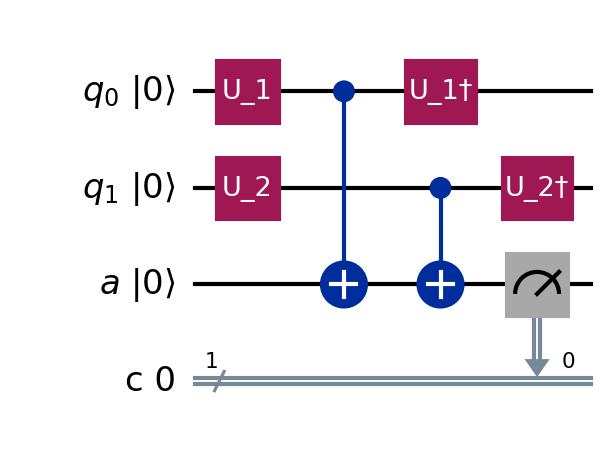
\includegraphics[width=0.7\linewidth]{figs/q6_b_pauli_measure}
\caption{任意 Pauli 算符 $P=P_1\otimes P_2$ 的投影测量模板：$U_i$（满足 $U_iP_iU_i^\dagger=Z$）$\to$ 奇偶校验 $\to$ $U_i^\dagger$ 复原。}
\end{figure}

\textbf{正确性。} 旋转后 $P$ 变为 $\widetilde{P}=\bigotimes_{i\in\mathrm{supp}} Z_i$，其本征值是支集上各 $Z$ 本征值之积。各 $\mathrm{CNOT}(i\to a)$ 把 $\ket{1}$ 的个数（即 $z_i=-1$ 的个数）累加到 $a$ 上，故 $a$ 的测量值 $m=\bigoplus_{i\in\mathrm{supp}} b_i$，而 $\widetilde P$ 的本征值 $=\prod_i z_i=(-1)^m$，恰由 $a$ 读出：$m=0\Rightarrow +1$，$m=1\Rightarrow -1$。$U_i^\dagger$ 把态转回原基，所以最终数据寄存器被投影到 $P$ 的 $\pm1$ 本征子空间，且不破坏子空间内的相干性。

\hfill $\square$

\medskip
\noindent\textbf{Solution (c).} 设保留第一个比特为目标，对其余 $n-1$ 个比特做 $X$（Hadamard）基测量并作经典前馈。初始态
\begin{equation*}
    \ket{\Psi_n}=\alpha\ket{0}_1\ket{0\cdots0}_{2..n}+\sqrt{1-\alpha^2}\,\ket{1}_1\ket{1\cdots1}_{2..n}.
\end{equation*}
\textbf{协议：} (i) 对比特 $2,\dots,n$ 各施加 $H$；(ii) 在计算基下测量 $2,\dots,n$，得 $b_2,\dots,b_n\in\{0,1\}$；(iii) 计算奇偶 $s=b_2\oplus\cdots\oplus b_n$，对比特 1 施加受经典控制的 $Z^s$（即 $s=1$ 时施加 $Z$）。完成后比特 1 即为 $\alpha\ket{0}+\sqrt{1-\alpha^2}\,\ket{1}$。

\begin{figure}[H]
\centering

\includegraphics[width=0.7\linewidth]{figs/q6_c_ghz_to_single}
\caption{（$n=3$ 示意）先制备 GHZ 态，再在 $X$ 基下测量 $q_1,q_2$，按奇偶 $s$ 对 $q_0$ 施加经典前馈 $Z^s$，即得 $\alpha\ket{0}+\sqrt{1-\alpha^2}\ket{1}$。}
\end{figure}

\textbf{推导。} 用 $\ket{\pm}=\frac{1}{\sqrt2}(\ket0\pm\ket1)$ 与
\begin{equation*}
    \ket{+\cdots+}=\tfrac{1}{\sqrt{2^{n-1}}}\!\!\sum_{b_2..b_n}\!\!\ket{b_2..b_n},\qquad
    \ket{-\cdots-}=\tfrac{1}{\sqrt{2^{n-1}}}\!\!\sum_{b_2..b_n}\!\!(-1)^{b_2+\cdots+b_n}\ket{b_2..b_n},
\end{equation*}
施 $H$ 后
\begin{equation*}
    \ket{\Psi_n}=\frac{1}{\sqrt{2^{n-1}}}\sum_{b_2..b_n}\Big(\alpha\ket{0}_1+(-1)^{s}\sqrt{1-\alpha^2}\,\ket{1}_1\Big)\ket{b_2..b_n}.
\end{equation*}
测量 $2,\dots,n$ 得任一具体结果时，比特 1 坍缩为（已归一化）$\alpha\ket{0}+(-1)^s\sqrt{1-\alpha^2}\,\ket{1}$。由于 $Z\ket{1}=-\ket{1}$，施加 $Z^s$ 恰好抵消 $(-1)^s$：
\begin{equation*}
    Z^s\big(\alpha\ket{0}+(-1)^s\sqrt{1-\alpha^2}\,\ket{1}\big)=\alpha\ket{0}+\sqrt{1-\alpha^2}\,\ket{1}.
\end{equation*}
\textbf{成功概率为 1（确定性）。} 每种测量结果都可用，只需前馈修正；各结果等概率 $1/2^{n-1}$。$n=2$ 特例：测量比特 2 于 $X$ 基，结果 $+1$（$s=0$）即得目标态，结果 $-1$（$s=1$）则补一个 $Z$。这正是“基于测量的纠缠式单比特态制备”。

\hfill $\square$

\medskip
\noindent\textbf{Solution (d) (Optional).} 在仅允许最近邻 $\mathrm{CNOT}(q_i,q_{i+1})$ 的路径上把 $q_0$ 扇出到 $q_1,\dots,q_4$。$F_4$ 作为可逆线性映射 $x_i\mapsto x_i\oplus x_0$（$i\ge1$，$q_0$ 不变）。由于是 $5$ 比特门，数据寄存器本身就是 $5$ 比特的下界；下面的幺正实现\textbf{不使用辅助比特}，并在规模上达到最优。

\textbf{规模最优幺正实现（阶梯/有限差分）。} 沿链下行做差分（telescope）、在 $q_0$ 注入 $x_0$、再上行重新累积，共用 $7$ 个最近邻 CNOT（深度 $7$）：
\begin{equation*}
\mathrm{CNOT}(3{\to}4),\ \mathrm{CNOT}(2{\to}3),\ \mathrm{CNOT}(1{\to}2),\ \mathrm{CNOT}(0{\to}1),\ \mathrm{CNOT}(1{\to}2),\ \mathrm{CNOT}(2{\to}3),\ \mathrm{CNOT}(3{\to}4).
\end{equation*}
\textbf{正确性。} 下行后各比特取差分形式 $q_i\gets x_i\oplus x_{i-1}$（$i=1,\dots,4$，最右端 $q_4\gets x_4\oplus x_3$），中央的 $\mathrm{CNOT}(0{\to}1)$ 把 $q_1$ 变为 $x_1\oplus x_0$；随后上行 $\mathrm{CNOT}(1{\to}2),(2{\to}3),(3{\to}4)$ 把差分逐级累加，得到 $q_i=x_i\oplus x_0$（$i=1,\dots,4$），$q_0=x_0$。该映射已对全部 $2^5=32$ 个计算基输入数值验证（见 \texttt{code/problem1\_measurement.py} 的 (d) 段）。

\begin{figure}[H]
\centering

\includegraphics[width=0.95\linewidth]{figs/q6_d_fanout_f4}
\caption{$F_4$ 扇出的\textbf{规模最优}幺正实现：$7$ 个最近邻 CNOT（阶梯结构），深度 $7$。}
\end{figure}

\textbf{最优性与深度下界（穷举证明）。} 把每个数据比特表示为原始输入在 $\mathbb F_2$ 上的线性型，对全部“有向匹配层”（一层内可并行的最近邻 CNOT 集合，共 $20$ 种）做分层 BFS：
\begin{itemize}
    \item \textbf{最小规模}：以单个 CNOT 为步的 BFS 给出最小 CNOT 数 $=7$，故上式规模最优；
    \item \textbf{最小深度}：分层 BFS 表明深度 $\le 5$ 时至多到达 $36464$ 个态且不含 $F_4$ 目标态，深度 $=6$ 才首次可达。\textbf{故最小深度为 $6$，深度 $4$ 不可达。}
\end{itemize}
光锥论证只给出 $\ge 4$，但扇出还要求中间比特被“洗净”（仅添 $x_0$、不引入前缀异或），需要信号传到末端后再传回，因此实际下界更高。规模与深度不可同时取到各自最小：深度 $6$ 的实现需 $10$ 个 CNOT，例如
\begin{equation*}
\begin{array}{l}
L_0:\ \mathrm{CNOT}(0{\to}1)\\
L_1:\ \mathrm{CNOT}(1{\to}0),\ \mathrm{CNOT}(3{\to}4)\\
L_2:\ \mathrm{CNOT}(0{\to}1),\ \mathrm{CNOT}(2{\to}3)\\
L_3:\ \mathrm{CNOT}(1{\to}2)\\
L_4:\ \mathrm{CNOT}(0{\to}1),\ \mathrm{CNOT}(2{\to}3)\\
L_5:\ \mathrm{CNOT}(1{\to}0),\ \mathrm{CNOT}(3{\to}4)
\end{array}
\end{equation*}
故 Pareto 前沿为 $(\text{规模},\text{深度})\in\{(7,7),(10,6)\}$：优化规模取阶梯实现，优化深度取上式。

\textbf{用测量进一步降深度。} 若额外允许\textbf{预先共享纠缠资源}（沿路径排布的 Bell 对或 GHZ 猫态），可用量子传态思路在 $O(1)$ 深度内实现远距离 CNOT：以猫态为媒介对辅助比特做联合（贝尔型）测量并按结果作经典前馈 Pauli 修正，可把扇出深度降到与 $n$ 无关；代价是 $O(n)$ 个辅助比特与预共享纠缠（注意：仅做单比特 $X$ 基测量并不足以完成，需两比特联合测量）。

\hfill $\square$

\medskip
\noindent\textbf{Solution (e) (Optional).} 用 \textbf{SWAP 检验}（swap test）。引入一个辅助比特 $c\ket{0}$，电路为：
\begin{equation*}
    \xrightarrow{H(c)}\ \xrightarrow{\mathrm{cSWAP}(c;\,\psi,\phi)}\ \xrightarrow{H(c)}\ \xrightarrow{\text{测 }c}.
\end{equation*}
其中受控交换 $\mathrm{cSWAP}$（Fredkin 门）可分解为 $2$ 个 $\mathrm{CNOT}$ 夹一个 Toffoli：$\mathrm{CNOT}(\psi,\phi)$；$\mathrm{Toffoli}(c,\phi,\psi)$；$\mathrm{CNOT}(\psi,\phi)$，而 Toffoli 又可由 $\mathrm{CNOT}+H$（$+T$ 门）实现。

\begin{figure}[H]
\centering
\begin{minipage}[t]{0.46\linewidth}\centering
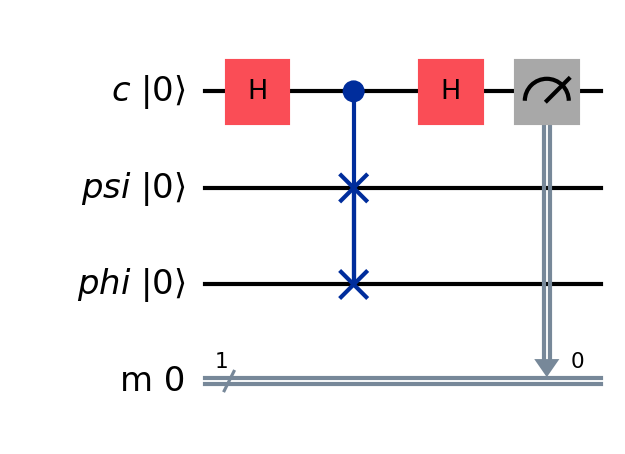
\includegraphics[width=\linewidth]{figs/q6_e_swap}\\[2pt]
{\footnotesize 高层：受控交换门}
\end{minipage}\hfill
\begin{minipage}[t]{0.49\linewidth}\centering
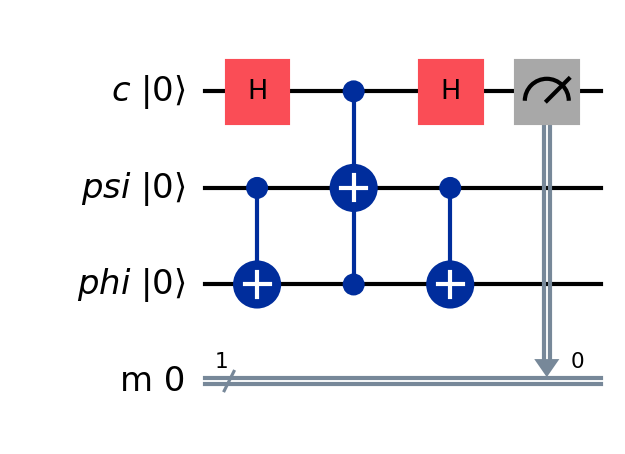
\includegraphics[width=\linewidth]{figs/q6_e_swap_decomposed}\\[2pt]
{\footnotesize 分解：$2\,\mathrm{CNOT}+\text{Toffoli}$}
\end{minipage}
\caption{SWAP 检验线路：左为受控交换门表示，右为 $2\,\mathrm{CNOT}+\text{Toffoli}$ 的门级分解。}
\end{figure}

\textbf{分析。} 第一个 $H$ 后 $c=\frac{1}{\sqrt2}(\ket0+\ket1)$；$\ket1$ 分支把 $\ket\psi,\ket\phi$ 交换。经第二个 $H$，
\begin{equation*}
    \braket{0|c}=\tfrac12\big(\ket{\psi}\ket{\phi}+\ket{\phi}\ket{\psi}\big),\qquad
    P(c=0)=\tfrac12\big(1+|\braket{\psi|\phi}|^2\big).
\end{equation*}
故
\begin{equation*}
    |\braket{\psi|\phi}|^2=2P(c=0)-1=1-2P(c=1),\qquad
    |\braket{\psi|\phi}|=\sqrt{\,2P(c=0)-1\,}.
\end{equation*}
多次重复统计 $P(c=0)$ 即可估计内积的模长。当 $\ket\psi=\ket\phi$ 时 $P(c=0)=1$；当二者正交时 $P(c=0)=\tfrac12$，符合预期。

\hfill $\square$

\subsection*{7. Reversible Circuit}
(Optional) Construct a reversible classical circuit using Toffoli and NOT gates to evaluate the formula:
\begin{align*}
    S_3(x) = &(\neg x_1 \lor \neg x_2) \land (x_1 \lor \neg x_2) \land (\neg x_1 \lor x_2 \lor \neg x_3) \\
             &\land (\neg x_1 \lor x_2 \lor x_3) \land (x_1 \lor x_2 \lor x_3),
\end{align*}
where each $x_i$ represents a Boolean value, and $\neg$, $\lor$, and $\land$ denote logical NOT, OR, and AND, respectively. Try to: (1) use as few ancillary qubits as possible, and (2) minimize the product of the number of gates and the total number of qubits.

\medskip
\noindent\textbf{Solution.}（实现见 \texttt{code/problem7\_reversible.py} 与 \texttt{code/quantum\_circuits.py}）

\textbf{化简。} 枚举 $S_3$ 的真值表可知，仅当 $(x_1,x_2,x_3)=(0,0,1)$ 时 $S_3=1$，其余情形均为 $0$，故
\begin{equation*}
    S_3(x)=\neg x_1 \wedge \neg x_2 \wedge x_3 .
\end{equation*}

\textbf{可逆线路（3 个 Toffoli + 4 个 NOT）。} 取 5 个量子比特：输入 $q_0,q_1,q_2$（对应 $x_1,x_2,x_3$）、辅助比特 $q_3=\text{anc}$、输出比特 $q_4=\text{result}$，均初始化为 $\ket{0}$。按顺序施加：
\begin{enumerate}[label=步骤\arabic*.]
    \item $X(q_0),\ X(q_1)$：翻转控制位，使得 $\neg x_1,\neg x_2$ 以 $1$ 表示；
    \item $\mathrm{Toffoli}(q_0,q_1\to q_3)$：$\text{anc}=\neg x_1\wedge\neg x_2$；
    \item $\mathrm{Toffoli}(q_3,q_2\to q_4)$：$\text{result}=\text{anc}\wedge x_3=S_3(x)$；
    \item $\mathrm{Toffoli}(q_0,q_1\to q_3)$：反计算，将辅助比特复位回 $\ket{0}$；
    \item $X(q_0),\ X(q_1)$：复位输入比特，还原 $x_1,x_2$。
\end{enumerate}
线路结束后 $q_4$ 存放 $S_3(x)$，其余比特（含辅助比特）均回到初值，因此线路是可逆且“干净”的。

\begin{figure}[H]
\centering

\includegraphics[width=0.9\linewidth]{figs/problem7_circuit.pdf}
\caption{$S_3(x)$ 的可逆线路：$4$ 个 NOT $+$ $3$ 个 Toffoli，共 $5$ 个量子比特（$3$ 输入 $+$ $1$ 辅助 $+$ $1$ 输出）。}
\end{figure}

\textbf{资源统计。} 门数 $=4\ \text{NOT}+3\ \text{Toffoli}=7$；量子比特数 $=3+1+1=5$；二者乘积 $=7\times5=35$。仅用 $1$ 个辅助比特。全部 $8$ 种输入的正确性已用 TensorCircuit 逐一验证通过（见 \texttt{problem7\_reversible.py} 的 \texttt{verify\_circuit}）。

\hfill $\square$

\subsection*{8. Grover Search}
(Optional) Using the results from the previous problem, find a configuration of $x$ satisfying $S_3(x) = \text{True}$ with Grover's search algorithm. Implement your algorithm using TensorCircuit and verify the solution.

\medskip
\noindent\textbf{Solution.}（实现见 \texttt{code/8\_grover.py}）

搜索空间为 $3$ 个数据比特，$N=2^3=8$，满足 $S_3(x)=\text{True}$ 的解唯一：$x=(0,0,1)$，即 $\ket{001}$，故解数 $M=1$。

\textbf{Oracle（相位翻转）。} 复用第 7 题的可逆线路 \texttt{build\_s3} 把 $S_3(x)$ 计算到输出比特 $q_4$，对 $q_4$ 施加 $Z$（当 $S_3=1$ 时贴上 $-1$ 相位），再次施加 \texttt{build\_s3} 反计算以清空 $q_4$ 与辅助比特 $q_3$：
\begin{equation*}
    O:\quad \texttt{build\_s3}\ \to\ Z(q_4)\ \to\ \texttt{build\_s3}.
\end{equation*}
效果为 $O\ket{x}=(-1)^{S_3(x)}\ket{x}$，且线路结束后所有辅助比特回到 $\ket{0}$。

\textbf{扩散算子（Diffusion）。} 在 $3$ 个数据比特上实现 $D=H^{\otimes3}(2\ket{000}\!\bra{000}-I)H^{\otimes3}$，即
\begin{equation*}
    D:\quad H^{\otimes3}\ \to\ X^{\otimes3}\ \to\ \mathrm{MCZ}(q_0,q_1,q_2)\ \to\ X^{\otimes3}\ \to\ H^{\otimes3},
\end{equation*}
其中多控 $Z$（MCZ）借用干净的辅助比特 $q_3$ 实现：$\mathrm{Toffoli}(q_0,q_1\to q_3)$，$H(q_2)$，$\mathrm{CNOT}(q_3\to q_2)$，$H(q_2)$，$\mathrm{Toffoli}(q_0,q_1\to q_3)$。

\textbf{迭代次数与结果。} 令 $\theta=\arcsin\sqrt{M/N}=\arcsin\sqrt{1/8}$，最优迭代次数
\begin{equation*}
    k_{\text{opt}}=\left\lfloor \frac{\arccos\sqrt{M/N}}{2\theta}\right\rfloor=2 .
\end{equation*}
初态取 $3$ 个数据比特上的均匀叠加 $H^{\otimes3}\ket{000}$，交替施加 $O$ 与 $D$ 共 $k_{\text{opt}}$ 次后，对数据比特测量，解 $\ket{001}$ 的概率显著放大到接近 $1$。TensorCircuit 数值验证表明最可能的输出即 $\ket{001}$，且代入 $S_3$ 校验为真（见 \texttt{8\_grover.py} 的 \texttt{verify}）。整个线路共 $5$ 个量子比特（$3$ 数据 $+\ 2$ 复用自第 7 题的辅助/输出比特）。

\hfill $\square$

\end{document}
